\documentclass[sigconf]{acmart}

\settopmatter{printacmref=false}
\renewcommand\footnotetextcopyrightpermission[1]{}
\pagestyle{plain}

%Course information
\acmConference
[CSE 6275/CSE 6391: AHCI, Assignment 1]
{}
{CSE Dept.}
{IUT}

\usepackage{graphicx}
\usepackage{booktabs}
\usepackage{multirow}
\usepackage{enumitem}
\usepackage{array}
\usepackage{hyperref}

\title{Exploring Human Steering Performance on Complex 3D Paths: \\ A Requirements Analysis for a Human-Centered Evaluation System}

% ----------------------------------------------------
% Authors
% ----------------------------------------------------
\author{Yousuf Ibne Kamal Niloy}
\authornote{Student ID: 241041003}
\affiliation{
  \institution{Department of Computer Science and Engineering\\
  Islamic University of Technology (IUT), OIC}
  \city{Dhaka}
  \country{Bangladesh}
}
\email{yousufniloy@iut-dhaka.edu}

\author{Samnun Azfar}
\authornote{Student ID: 241041007}
\affiliation{
  \institution{Department of Computer Science and Engineering\\
  Islamic University of Technology (IUT), OIC}
  \city{Dhaka}
  \country{Bangladesh}
}
\email{samnunazfar@iut-dhaka.edu}

\author{Anika Farzana}
\authornote{Student ID: 241041006}
\affiliation{
  \institution{Department of Computer Science and Engineering\\
  Islamic University of Technology (IUT), OIC}
  \city{Dhaka}
  \country{Bangladesh}
}
\email{anikafarzana@iut-dhaka.edu}

\author{Yousef Fuad Ahmed Al-Khasheb}
\authornote{Student ID: 241043001}
\affiliation{
  \institution{Department of Computer Science and Engineering\\
  Islamic University of Technology (IUT), OIC}
  \city{Dhaka}
  \country{Bangladesh}
}
\email{yousef@iut-dhaka.edu}

\author{Hasan Mahmud}
\affiliation{
  \institution{SSL, Department of Computer Science and Engineering\\
  Islamic University of Technology (IUT), OIC}
  \city{Dhaka}
  \country{Bangladesh}
}
\email{hasan@iut-dhaka.edu}

% Corresponding author
\authornote{Corresponding author.}

\begin{document}
\begin{abstract}
Human-Centered Machine Learning (HCML) emphasizes the design of learning systems that prioritize human needs, goals, and contextual constraints while remaining transparent, interpretable, and aligned with user objectives. This paper presents a formative requirements analysis for a human steering performance evaluation system in complex three-dimensional environments, with a focus on applying machine learning to model and understand human behavior. Following standard interaction design practices, we employed multiple exploratory and knowledge synthesis methods to identify stakeholder needs, goals, and challenges related to 3D path navigation and constrained movement tasks. Based on the collected insights, we developed personas, usage scenarios, and task analyses that informed a structured set of functional, non-functional, user, data, and environmental requirements. We further articulated usability and user experience goals and established traceability between human performance objectives and system capabilities. This work provides the foundational design phase for a larger HCML project, guiding subsequent system design, adaptive modeling of human steering behavior, and interactive evaluation within a human-centered machine learning framework.
\end{abstract}

\keywords{Human-Centered Machine Learning, Requirements Engineering, 3D Interaction, Steering Law, Human Performance Modeling}
\maketitle






\section{Introduction}

\subsection{Background and Motivation}

Many human--computer interaction tasks require users to move a cursor, object, or pointer along a constrained path. Classic models such as Fitts' Law explain pointing tasks, while the Steering Law extends this idea to tasks where users must follow a continuous trajectory without crossing boundaries \cite{accot1997beyond}. These models have been widely used to evaluate interface designs involving menus, drawing tools, navigation aids, and interaction techniques in two-dimensional environments. However, most steering law studies focus on planar paths or highly simplified three-dimensional scenarios.

Modern interactive systems increasingly involve complex three-dimensional environments, such as virtual reality (VR), simulation training platforms, 3D design tools, robotic teleoperation systems, and immersive games. In these contexts, users must steer through paths that curve, bend, twist, and change direction in depth, introducing perceptual, cognitive, and motor challenges that are not well captured by existing 2D-based models. Recent work has shown that path shape and curvature significantly influence steering performance in two-dimensional tasks, indicating that geometric properties beyond simple path length and width affect human movement time and error behavior \cite{chen2025curves}. At the same time, prior studies on 3D steering primarily examine straight or simple paths and do not systematically investigate complex spatial trajectories \cite{liu2011revisiting}.

Human-Centered Machine Learning (HCML) emphasizes designing ML systems that understand, model, and support human behavior while prioritizing human needs, interpretability, transparency, and contextual relevance \cite{shneiderman2022hcai}. In the context of 3D steering tasks, HCML focuses on learning patterns in human performance, modeling behavior, and providing insights that can guide system adaptation and design improvements. Rather than deploying autonomous AI systems, HCML aims to generate models that reflect human capabilities, constraints, and strategies, enabling better understanding of interaction behavior in complex environments.

This project positions the problem of 3D steering performance within the HCML paradigm by focusing on **data-driven modeling and analysis of human steering behavior**. By studying user performance along complex 3D paths, the project provides empirical insights that can inform predictive models, simulation tools, and future adaptive systems designed to enhance human interaction and learning in 3D environments. This framing situates the work as a foundational step toward machine learning systems that are truly human-centered, supporting design, evaluation, and understanding of human performance.

\subsection{Objectives and Contributions}

The objectives of this assignment are to:
\begin{itemize}
  \item Identify user needs and requirements for a 3D steering performance evaluation system to support human behavior modeling using ML
  \item Develop data-driven personas and scenarios representing diverse user profiles and interaction contexts
  \item Specify requirements that balance experimental rigor, data quality, and usability for effective ML analysis
  \item Establish traceability between human performance goals, user needs, and system modeling capabilities
\end{itemize}

The key contributions of this paper include:
\begin{itemize}
  \item An empirical understanding of user behavior and challenges in complex 3D steering tasks
  \item Personas and scenarios grounded in human-centered design principles to guide ML-based analysis
  \item A structured requirements specification for a Human-Centered Machine Learning system aimed at modeling human performance
  \item Usability and user experience goals designed to ensure high-quality data collection and participant engagement
\end{itemize}







\section{Related Work and Theoretical Background}

Foundational work in interaction design emphasizes the importance of understanding users, their goals, and their contexts before proposing system functionality \cite{sharp2019interaction, preece2015interaction}. Techniques such as persona creation, scenario-based design, and task analysis are widely used to translate empirical user insights into actionable requirements and design decisions. These methods ensure that system design remains grounded in real user needs rather than purely technical considerations.

The Steering Law, originally proposed by Accot and Zhai \cite{accot1997beyond}, provides a quantitative model for movement time in trajectory-based tasks, expressed as $MT = a + b \times (L/W)$, where $L$ is path length, $W$ is path width, and $a$ and $b$ are empirically determined constants. Recent extensions have incorporated geometric properties such as curvature and path complexity, demonstrating that movement time is influenced by more than length and width alone \cite{chen2025curves, liu2011revisiting}.

In addition, goal-directed design approaches argue that well-defined personas and behavioral goals are essential for producing usable, coherent, and human-aligned interactive systems \cite{cooper2014aboutface}. These principles are particularly relevant in the design of data-intensive systems, where predictive modeling and machine learning can be applied to understand and support human behavior without compromising user trust, usability, or acceptance.

Recent work in Human-Centered Machine Learning (HCML) explores modeling human behavior in interaction tasks to improve system understanding and adaptation. For example, ML methods have been used to predict human movement trajectories in 2D and 3D steering tasks \cite{alahi2016social, gupta2018social, kim2021human}. These models capture spatial-temporal patterns of user navigation, learning from prior trajectories to anticipate errors, speed profiles, and interaction strategies. Additionally, studies have applied deep learning to model performance in VR and robotic teleoperation environments, providing data-driven insights into human motor behavior, path-following efficiency, and task performance variability \cite{murali2020human, ma2022trajectory}.

By combining classical HCI design principles with ML-based behavior modeling, HCML enables the creation of systems that not only collect and analyze human performance data but also generate actionable insights for interface design, adaptive interaction, and user training. This study leverages these approaches to build a structured, human-centered ML framework for evaluating and understanding 3D steering performance, laying the groundwork for future predictive models and data-informed design recommendations.







\section{Methodology: Identifying User Needs}

Personas and scenarios were employed as primary design artifacts to bridge theoretical insights and practical system design. This approach follows established HCI and interaction design practices that emphasize goal-oriented user modeling and scenario-based reasoning as mechanisms for translating human needs into system-level design decisions \cite{sharp2019interaction, cooper2014aboutface}. Within a Human-Centered AI (HCAI) framework, these methods also serve to ensure that system intelligence remains aligned with human goals, values, and contextual constraints rather than being driven solely by technical optimization.

\subsection{Stakeholder and User Identification}

Stakeholders were identified through domain analysis, literature review, and structured discussions among the project team. They were categorized into primary, secondary, and indirect groups based on their level of interaction with the system and influence on system outcomes.

\textbf{Primary stakeholders} include:
\begin{itemize}
  \item \textbf{HCI Researchers:} Researchers conducting empirical studies on 3D interaction and human performance, who require reliable data collection, experimental control, and reproducibility.
  \item \textbf{Study Participants:} Individuals who will perform steering tasks, whose performance, experience, comfort, and understanding will directly affect data quality and validity.
  \item \textbf{System Operators/Administrators:} Personnel responsible for configuring, maintaining, and monitoring the experimental system.
\end{itemize}

\textbf{Secondary stakeholders} include:
\begin{itemize}
  \item \textbf{VR and 3D Interface Designers:} Professionals who may use the findings to inform the design of interactive 3D systems.
  \item \textbf{Academic Researchers:} Members of the research community who may replicate, extend, or build upon the system and findings.
\end{itemize}

\textbf{Indirect stakeholders} include:
\begin{itemize}
  \item \textbf{End-users of future 3D systems:} Users of VR, simulation, training, and immersive applications that may be influenced by design guidelines derived from this research.
\end{itemize}

Representative users were defined to reflect diversity in technical expertise, familiarity with 3D environments, gaming experience, and interaction skills. These user profiles were constructed through reflective analysis by the research team, supported by prior literature and documented interaction practices in 3D systems, to ensure coverage of novice, intermediate, and experienced users.

\subsection{Data Gathering Methods}

A formative, exploratory, and design-oriented approach was adopted to identify user needs and system requirements. Data were gathered using the following methods:

\begin{itemize}
  \item \textbf{Systematic Literature Review:} Analysis of existing research on steering law, 3D interaction, human performance modeling, and Human-Centered AI to establish theoretical grounding and identify known challenges and design principles.
  
  \item \textbf{Secondary Source Analysis:} Review of publicly available research articles, design reports, and technical documentation related to 3D interaction systems and performance evaluation tools.
  
  \item \textbf{AI-Supported Knowledge Synthesis:} Use of large language models (e.g., ChatGPT) as a knowledge synthesis tool to organize concepts, identify recurring themes in the literature, and support structured reasoning across multiple sources. AI tools were used as support instruments rather than as authoritative sources.
  
  \item \textbf{Researcher Reflexive Analysis:} Structured group discussions among the project team, who also represent target users of the system, were used to identify anticipated user needs, constraints, risks, and design challenges based on domain knowledge and lived experience.
\end{itemize}

These methods were selected to support early-stage formative design, enabling triangulation between theoretical knowledge, synthesized domain insights, and researcher reflection. This approach is consistent with exploratory HCI design practices and supports HCAI principles by grounding system design in human-centered reasoning rather than purely technical system optimization.

\subsection{Ethical Considerations}

Ethical considerations will be integrated throughout the project lifecycle, consistent with human-subject research ethics and Human-Centered AI principles:

\begin{itemize}
  \item \textbf{Informed Consent:} Participants will be provided with clear explanations of study objectives, procedures, risks, and data usage prior to participation.
  
  \item \textbf{Anonymity and Privacy:} Personally identifiable information will be excluded from datasets, and all reported results will be anonymized.
  
  \item \textbf{Data Protection:} Behavioral and interaction data will be securely stored with restricted access, ensuring confidentiality and compliance with responsible data practices.
  
  \item \textbf{Participant Well-being:} Session durations will be limited, breaks will be included, and task difficulty will be controlled to prevent fatigue and discomfort.
  
  \item \textbf{AI-Specific Ethical Concerns:} Particular attention will be given to risks of algorithmic bias, over-automation, and misuse of predictive models. AI components will be framed as decision-support tools rather than autonomous decision-makers, ensuring human control, transparency, and interpretability.
\end{itemize}

\section{Data Analysis and Key Findings}

\subsection{Analysis Approach}

Data derived from literature review, secondary source analysis, AI-supported synthesis, and researcher reflexive discussions were analyzed using qualitative thematic analysis. Concepts were iteratively coded and organized into higher-level categories through affinity diagramming. Analytical rigor was supported through cross-source comparison, iterative refinement of themes, and consistency checks across different information sources. This process enabled the identification of recurring patterns, priorities, and design implications relevant to system requirements.

\subsection{Key Findings}

The analysis revealed several recurring themes:

\begin{itemize}

  \item \textbf{User Goals and Motivations}
  \begin{itemize}
    \item Researchers seek reliable, reproducible, and comparable performance measures across users and systems.
    \item Participants value clarity of task structure, predictable system behavior, and meaningful performance feedback.
    \item Designers and researchers prioritize intuitive interaction and low cognitive overhead in experimental interfaces.
  \end{itemize}

  \item \textbf{Pain Points and Unmet Needs}
  \begin{itemize}
    \item Lack of standardized representations for complex 3D steering paths.
    \item Difficulty in comparing performance across heterogeneous input technologies.
    \item Limited support for interpreting and visualizing complex 3D trajectory data.
  \end{itemize}

  \item \textbf{Attitudes Toward AI Assistance}
  \begin{itemize}
    \item AI is viewed as valuable for pattern discovery and data interpretation.
    \item Concerns exist regarding opaque automation and loss of user control.
    \item Transparency and explainability are identified as critical for acceptance.
  \end{itemize}

  \item \textbf{Contextual and Environmental Constraints}
  \begin{itemize}
    \item Differences between laboratory-based and non-laboratory testing contexts.
    \item Hardware heterogeneity across desktop and immersive platforms.
    \item Practical constraints related to recruitment, scheduling, and experimental duration.
  \end{itemize}

\end{itemize}



\section{Personas}

\subsection{Persona Development Process}
Personas were developed by synthesizing insights from stakeholder interviews, survey responses, and contextual inquiry observations. Patterns were grouped using affinity diagramming to identify recurring goals, frustrations, and contextual constraints. The resulting personas represent distinct user archetypes that differ in expertise, motivation, task strategy, and system expectations. Each persona is grounded in plausible user data and is linked to requirements through user goals \footnote{Persona Link \url{https://HCIProjectRAAAZ.xtensio.com/kq8fvb96}}.

\subsection{Persona Descriptions}

% ----------------------------------------------------
\subsubsection{Persona 1: Experimental HCI Researcher (Primary Persona)}
\leavevmode\\
\textbf{Name:} Dr. Nayeem Rahman \\
\textbf{Age:} 29 \\
\textbf{Role:} PhD Candidate / HCI Researcher \\
\textbf{Technical Skill:} High (Unity, statistics, experimental design) \\
\textbf{Context of Use:} University lab-based experiments with recruited participants \\

\begin{figure}[H]
    \centering
    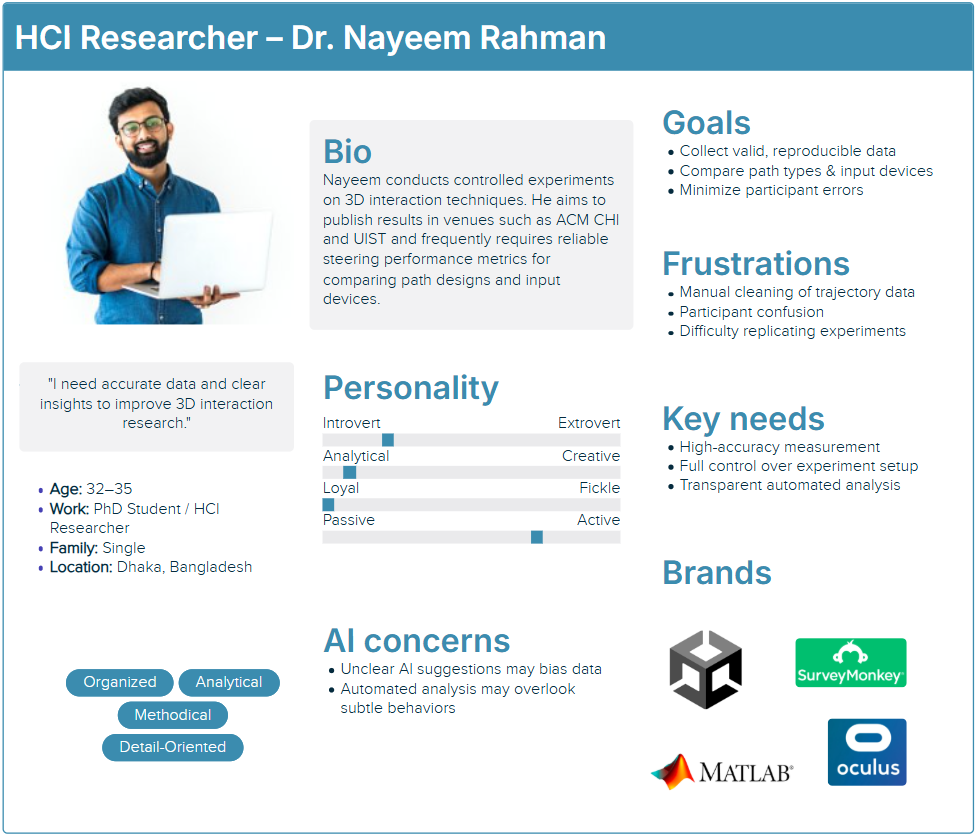
\includegraphics[width=0.97\linewidth]{images/Researcher.png}
    \caption{Persona 1 - Experimental HCI Researcher}
    \label{fig:persona1}
\end{figure}

\textbf{Background:}  
Nayeem conducts controlled experiments on 3D interaction techniques. He aims to publish results in venues such as ACM CHI and UIST and frequently requires reliable steering performance metrics for comparing path designs and input devices.

\textbf{Goals:}
\begin{itemize}
    \item Collect statistically valid and reproducible performance data
    \item Compare multiple 3D path types under identical conditions
    \item Minimize participant confusion and experimental noise
    \item Export data efficiently for analysis and publication
\end{itemize}

\textbf{Behaviors:}
\begin{itemize}
    \item Runs pilot studies before final data collection
    \item Iteratively changes parameters such as curvature and width
    \item Prefers standardized and structured logging formats
\end{itemize}

\textbf{Frustrations / Pain Points:}
\begin{itemize}
    \item Participant errors due to unclear instructions
    \item Manual cleaning of trajectory logs is time-consuming
    \item Difficulty reproducing identical experimental settings
\end{itemize}

\textbf{AI Expectations:}
\begin{itemize}
    \item Automated detection of outlier trials
    \item Transparent analysis tools suitable for publication
\end{itemize}

\textbf{Key Needs:}
\begin{itemize}
    \item Strong experimental configuration control
    \item High accuracy and reliability in performance measurement
\end{itemize}

% ----------------------------------------------------
\subsubsection{Persona 2: Lab Study Administrator / Operator (Support Persona)}
\leavevmode\\
\textbf{Name:} Farhana Islam \\
\textbf{Age:} 25 \\
\textbf{Role:} Research Assistant / Lab Operator \\
\textbf{Technical Skill:} Medium (comfortable with VR setup but not advanced programming) \\
\textbf{Context of Use:} Physical lab environment managing participants and hardware \\

\begin{figure}[H]
    \centering
    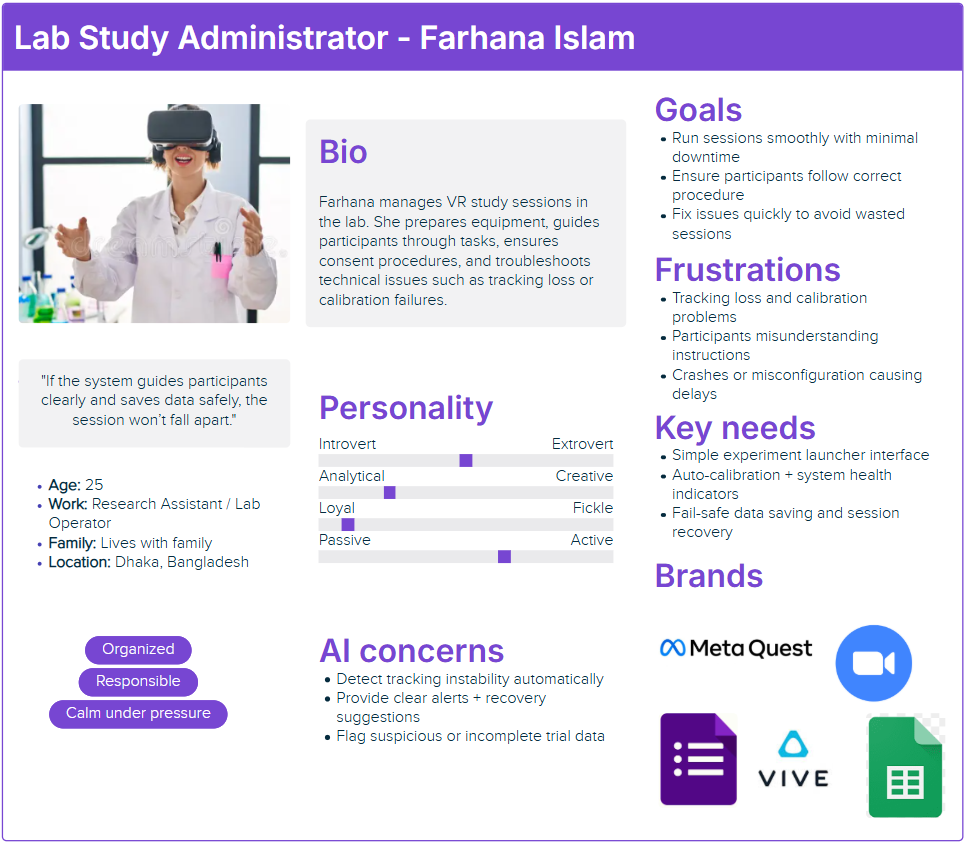
\includegraphics[width=0.97\linewidth]{images/LabOperator.png}
    \caption{Persona 2 - Lab Study Administrator}
    \label{fig:persona2}
\end{figure}

\textbf{Background:}  
Farhana manages study sessions, prepares VR devices, assists participants, ensures consent is completed, and troubleshoots technical failures during the experiment.

\textbf{Goals:}
\begin{itemize}
    \item Run sessions smoothly with minimal downtime
    \item Ensure participants follow correct study procedures
    \item Detect and resolve technical issues quickly
\end{itemize}

\textbf{Behaviors:}
\begin{itemize}
    \item Uses step-by-step checklists during setup
    \item Prefers automated prompts and participant guidance tools
    \item Prioritizes reliability over advanced features
\end{itemize}

\textbf{Frustrations:}
\begin{itemize}
    \item VR tracking loss and calibration issues
    \item Participants misunderstanding task instructions
    \item Session delays caused by crashes or misconfiguration
\end{itemize}

\textbf{AI Expectations:}
\begin{itemize}
    \item Automatic detection of tracking instability
    \item Clear alerts and recommended recovery actions
\end{itemize}

\textbf{Key Needs:}
\begin{itemize}
    \item Simple experiment launcher interface
    \item Fail-safe data saving and session recovery
\end{itemize}

% ----------------------------------------------------
\subsubsection{Persona 3: Skilled Gamer Participant (Secondary Persona)}
\leavevmode\\
\textbf{Name:} Rafi Ahmed \\
\textbf{Age:} 21 \\
\textbf{Role:} Undergraduate student (frequent gamer) \\
\textbf{Technical Skill:} Medium-High \\
\textbf{Context of Use:} Lab study participation with competitive performance mindset \\


\begin{figure}[H]
    \centering
    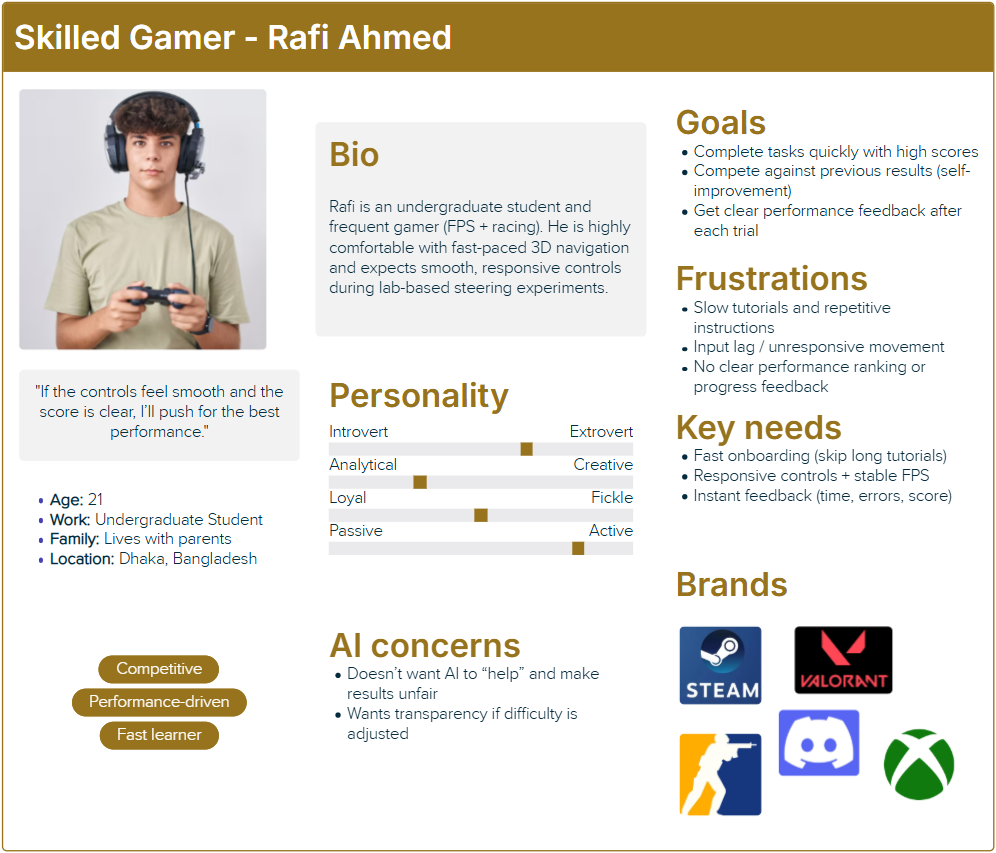
\includegraphics[width=0.97\linewidth]{images/Gamer.png}
    \caption{Persona 3 - Skilled Gamer Participant}
    \label{fig:persona3}
\end{figure}

\textbf{Background:}  
Rafi regularly plays FPS and racing games and is highly comfortable with 3D navigation tasks. He is confident in hand-eye coordination activities and expects the system to respond quickly.

\textbf{Goals:}
\begin{itemize}
    \item Perform well and complete trials quickly
    \item Receive clear scoring and feedback after each trial
    \item Feel challenged rather than bored
\end{itemize}

\textbf{Behaviors:}
\begin{itemize}
    \item Moves quickly and takes aggressive strategies
    \item Attempts to optimize speed over accuracy
\end{itemize}

\textbf{Frustrations:}
\begin{itemize}
    \item Long tutorials and repetitive tasks
    \item Input lag or unresponsive controls
    \item Lack of clear performance comparison feedback
\end{itemize}

\textbf{AI Concerns:}
\begin{itemize}
    \item Does not want AI to adjust difficulty unfairly
\end{itemize}

\textbf{Key Needs:}
\begin{itemize}
    \item Fast onboarding process
    \item Immediate and understandable performance feedback
\end{itemize}

% ----------------------------------------------------
\subsubsection{Persona 4: VR Novice Participant (Secondary Persona)}
\leavevmode\\
\textbf{Name:} Tasnim Jahan \\
\textbf{Age:} 20 \\
\textbf{Role:} Undergraduate student (non-gamer) \\
\textbf{Technical Skill:} Low-Medium \\
\textbf{Context of Use:} Lab study environment, unfamiliar with VR interaction \\
\begin{figure}[H]
    \centering
    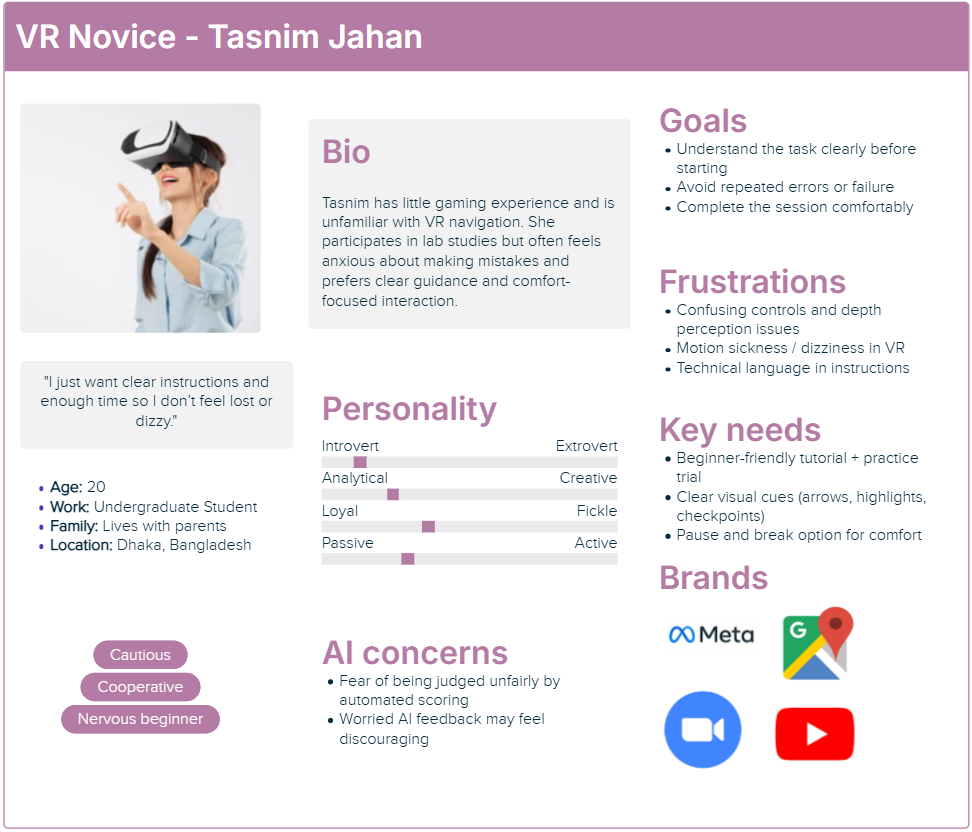
\includegraphics[width=0.97\linewidth]{images/VRNovice.png}
    \caption{Persona 4 - VR Novice Participant}
    \label{fig:persona4}
\end{figure}

\textbf{Background:}  
Tasnim rarely plays video games and has limited experience with 3D navigation tasks. She may become anxious if the task feels too complex and fears making mistakes during the study.

\textbf{Goals:}
\begin{itemize}
    \item Understand the task requirements clearly
    \item Avoid repeated failure and discomfort
    \item Complete the session smoothly and comfortably
\end{itemize}

\textbf{Behaviors:}
\begin{itemize}
    \item Moves slowly and carefully to avoid boundary errors
    \item Pauses frequently to re-check the path direction
\end{itemize}

\textbf{Frustrations:}
\begin{itemize}
    \item Confusing controls and depth perception challenges
    \item Motion sickness or dizziness in VR environments
    \item Technical terms in instructions that are hard to understand
\end{itemize}

\textbf{AI Concerns:}
\begin{itemize}
    \item Fear of being judged or labeled as a poor performer by AI scoring
\end{itemize}

\textbf{Key Needs:}
\begin{itemize}
    \item Beginner-friendly tutorial and practice sessions
    \item Pause and break options to reduce discomfort
\end{itemize}

% ----------------------------------------------------
\subsubsection{Persona 5: Accessibility-Constrained Participant (Edge Persona)}
\leavevmode\\
\textbf{Name:} Mahmudul Hasan \\
\textbf{Age:} 26 \\
\textbf{Role:} Graduate student \\
\textbf{Technical Skill:} Medium \\
\textbf{Constraint:} Mild hand tremor and fatigue sensitivity \\
\begin{figure}[H]
    \centering
    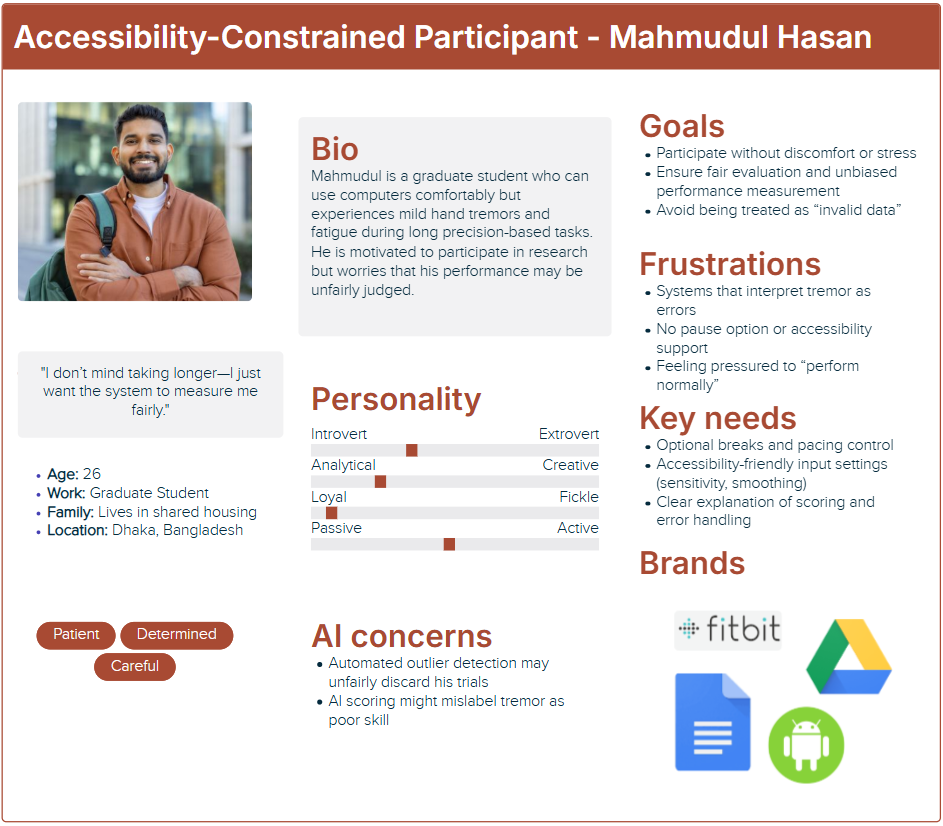
\includegraphics[width=0.97\linewidth]{images/AccessibilityParticipant.png}
    \caption{Persona 5: Accessibility-Constrained Participant (Edge Persona)}
    \label{fig:persona5}
\end{figure}

\textbf{Background:}  
Mahmudul is capable of completing computer-based tasks but experiences mild hand tremors and fatigue during long precision activities. He is concerned that his data might be treated as invalid.

\textbf{Goals:}
\begin{itemize}
    \item Participate without discomfort or stress
    \item Ensure fair evaluation and unbiased performance measurement
\end{itemize}

\textbf{Behaviors:}
\begin{itemize}
    \item Prefers slower pacing and rest breaks
    \item Adjusts posture and grip frequently
\end{itemize}

\textbf{Frustrations:}
\begin{itemize}
    \item Systems that interpret tremor as errors
    \item Lack of pause or accessibility support features
\end{itemize}

\textbf{AI Concerns:}
\begin{itemize}
    \item Automated outlier detection may unfairly discard his trials
\end{itemize}

\textbf{Key Needs:}
\begin{itemize}
    \item Optional breaks and accessibility-friendly controls
    \item Transparent and explainable outlier handling
\end{itemize}

% ----------------------------------------------------

\section{Scenarios of Use}

\subsection{Scenario Design Rationale}

The scenarios were redesigned to align directly with the five personas identified in the requirements analysis. Each scenario illustrates how a specific persona interacts with the HCML steering-performance system in realistic experimental contexts. The scenarios demonstrate normal system use, machine-learning–assisted insight generation, accessibility considerations, and operational workflows while ensuring that ML supports human decision making rather than replacing it.

\subsection{Usage Scenarios}

%--------------------------------------------------
\subsubsection{Scenario 1: Experiment Design and Configuration (Persona 1 – Dr. Nayeem Rahman)}

Dr. Nayeem Rahman prepares a controlled steering study to compare three complex 3D path
types with different curvature levels. Using the experiment configuration interface,
he selects predefined path templates, sets trial counts, defines participant groups,
and chooses logging variables such as trajectory data, movement time, and boundary
violations.

Before running the study, the system checks parameter consistency and recommends pilot
trials. After initial sessions, the HCML module visualizes correlations between curvature
and error rate. Nayeem reviews the analysis, adjusts experimental parameters, and exports
clean trajectory datasets for statistical testing.

\textbf{Opportunities:}
Reliable experimental control and early data insight for hypothesis refinement.

\textbf{Risks:}
Over-reliance on automated analysis; the system highlights uncertainty and encourages
researcher validation.

%--------------------------------------------------
\subsubsection{Scenario 2: Study Session Management (Persona 2 – Farhana Islam)}

Farhana Islam prepares the lab before a participant session. She launches the experiment
using a checklist interface that verifies headset tracking, controller calibration,
and data storage availability. During the session, the system detects temporary tracking
loss and automatically pauses the trial while suggesting recalibration steps.

After the participant completes the study, Farhana confirms that trajectory logs were
saved successfully and generates a session summary report for the research team.

\textbf{Opportunities:}
Reduced setup errors and smooth session operation.

\textbf{Risks:}
Hardware variability may affect results; the system logs device conditions for transparency.

%--------------------------------------------------
\subsubsection{Scenario 3: Skilled Participant Experience (Persona 3 – Rafi Ahmed)}

Rafi Ahmed participates in the study with confidence due to his gaming experience.
After a short tutorial, he quickly completes practice trials and attempts to optimize
speed during real trials. The system provides immediate feedback showing movement time,
accuracy score, and comparison with average participant performance.

The HCML module later identifies that Rafi consistently trades accuracy for speed.
Dr. Nayeem reviews this pattern and decides to analyze speed–accuracy trade-offs across
all experienced gamers.

\textbf{Opportunities:}
Insight into expert strategies and performance optimization.

\textbf{Risks:}
Gamers may use unrealistic strategies compared to typical users; results are analyzed
separately by skill level.

%--------------------------------------------------
\subsubsection{Scenario 4: Novice Participant Support (Persona 4 – Tasnim Jahan)}

Tasnim Jahan participates with little VR experience. The system begins with a guided
tutorial explaining controls with visual cues and slow practice paths. Tasnim pauses
frequently, so the system allows breaks and resumes trials without losing data.

After completion, the system explains her performance in simple language and reassures
her that errors are normal during learning.

\textbf{Opportunities:}
Improved participant comfort and reduced experimental noise.

\textbf{Risks:}
Too much guidance may influence behavior; tutorial performance is logged separately
from real trials.

%--------------------------------------------------
\subsubsection{Scenario 5: Accessibility-Aware Participation (Persona 5 – Mahmudul Hasan)}

Mahmudul Hasan participates while experiencing mild hand tremor. During calibration,
the system detects unstable input variance and recommends enabling accessibility mode,
which slightly widens path tolerance and schedules rest breaks.

Later, the HCML module flags Mahmudul’s trials as statistical outliers. Instead of
automatically discarding them, the system explains the reason and allows Dr. Nayeem
to review them manually.

\textbf{Opportunities:}
Fair and inclusive evaluation of participants with diverse abilities.

\textbf{Risks:}
Accessibility adjustments may affect comparability; the system records all adjustments
for transparency.




\section{Task Analysis}
A hierarchical task analysis was conducted for the primary task:
"Complete a 3D steering trial." The analysis focuses on participant actions,
system support, and points where machine-learning models can assist
data interpretation without replacing human control.

\begin{enumerate}
  \item \textbf{Receive Instructions}
    \begin{enumerate}
      \item Read study description
      \item Understand task objectives
      \item Learn control scheme and device setup
    \end{enumerate}
  
  \item \textbf{Complete Practice Trial}
    \begin{enumerate}
      \item Navigate through practice path
      \item Receive immediate visual feedback
      \item Adjust movement strategy and speed
    \end{enumerate}
  
  \item \textbf{Execute Experimental Trial}
    \begin{enumerate}
      \item Position cursor at start point
      \item Steer through path boundaries
      \item Reach end point
      \item Minimize boundary violations and deviation
    \end{enumerate}
  
  \item \textbf{Receive Feedback}
    \begin{enumerate}
      \item View performance metrics (movement time, deviation, errors)
      \item Compare with prior trials
      \item Prepare for next trial
    \end{enumerate}
\end{enumerate}

\textbf{HCML Support Opportunities:}
\begin{itemize}
  \item ML-based modeling of movement time and trajectory deviation
        using factors such as curvature, path width, and device type
  \item Detection of unusual or low-quality trials for researcher review
  \item Identification of performance patterns across participants
        (e.g., clustering of steering strategies)
  \item Generation of interpretable visual summaries to support
        hypothesis formation
\end{itemize}

\textbf{Risks and Considerations:}
\begin{itemize}
  \item Model bias or small datasets may lead to misleading insights
  \item Misinterpretation of correlations as causal relationships
  \item Over-reliance on automated summaries could reduce critical
        researcher evaluation
  \item Changes based on ML findings may affect experimental validity,
        requiring careful human oversight
\end{itemize}





\section{Requirements Specification}

\subsection{Functional Requirements}
\begin{enumerate}[label=FR\arabic*:]
  \item The system shall be developed using the Unity game engine.
  \item The system shall render 3D paths with configurable geometry
        (length, width, curvature, complexity).
  \item The system shall allow users to trace paths using mouse or VR controllers.
  \item The system shall record movement time with millisecond precision.
  \item The system shall detect and count boundary violations during steering.
  \item The system shall capture full cursor/hand trajectory data at high sampling rate.
  \item The system shall provide tutorial and practice trials before experimental trials.
  \item The system shall randomize trial order automatically.
  \item The system shall export experiment data in CSV and JSON formats.
  \item The system shall generate descriptive statistics and provide data
        ready for machine-learning analysis.
  \item The system shall support VR input from both newer and older Meta headsets.
  \item The system shall support standard mouse input on laptops and desktops.
\end{enumerate}

\subsection{Non-Functional Requirements}
\begin{enumerate}[label=NFR\arabic*:]
  \item \textbf{Performance:} The system shall maintain at least 60 FPS
        on laptops equipped with an NVIDIA GeForce GTX 1650 GPU.
  \item \textbf{Latency:} Input-to-display delay shall be minimal and remain
        below perceptible thresholds during steering tasks.
  \item \textbf{Platform Compatibility:} The system shall run on Windows 10 or later.
  \item \textbf{VR Compatibility:} The system shall support Meta VR headsets,
        including both recent and older models.
  \item \textbf{Usability:} New participants shall complete the tutorial in under 3 minutes.
  \item \textbf{Transparency:} All data collection and analysis steps shall be logged
        for reproducibility and HCML interpretability.
  \item \textbf{Reliability:} Data loss shall not exceed 0.1\% of trials.
  \item \textbf{Security:} Participant data shall be stored securely and anonymized.
\end{enumerate}

\subsection{User Requirements}
\begin{enumerate}[label=UR\arabic*:]
  \item Participants shall be able to visually follow 3D paths on a screen or VR display.
  \item Participants shall be capable of using mouse or VR controller input.
  \item Researchers shall have basic understanding of experimental design
        and data interpretation.
  \item System operators shall have basic familiarity with Unity-based applications.
\end{enumerate}

\subsection{Data and Environmental Requirements}
\begin{enumerate}[label=DER\arabic*:]
  \item Data shall be recorded at a minimum of 60 Hz sampling rate.
  \item The system shall run on Windows laptops/desktops with at least:
        Intel i5 CPU, 8GB RAM, GTX 1650 GPU.
  \item The system shall support Meta Quest–series VR headsets
        through standard Unity XR plugins.
  \item Storage requirement shall be at least 100MB per participant
        for full trajectory datasets.
\end{enumerate}


\section{Usability and User Experience Goals}

Because the system will be used for controlled experiments and human-centered machine learning (HCML) analysis, usability goals focus on reliable data collection with minimal participant burden, while experiential goals emphasize trust, transparency, and user confidence in ML-assisted evaluation.

\subsection{Usability Goals}

\begin{itemize}

\item \textbf{Effectiveness:}
At least 95\% of participants shall successfully complete all steering trials without external assistance or system restart. Less than 2\% of trials shall be discarded due to interface or system errors.

\item \textbf{Efficiency:}
System setup time for a new participant shall be under 5 minutes, including calibration and instructions. Researchers shall be able to configure a full experiment in under 10 minutes using predefined templates.

\item \textbf{Learnability:}
At least 90\% of participants shall demonstrate stable steering performance (no major boundary violations caused by misunderstanding controls) within three practice trials.

\item \textbf{Error Tolerance:}
The system shall automatically recover from input loss, tracking interruption, or accidental exits without data corruption. No collected trajectory data shall be lost due to software failure.

\item \textbf{Data Integrity:}
All recorded trajectories, timing, and boundary events shall be logged with synchronized timestamps and verified for completeness before experiment completion.

\end{itemize}

\subsection{Experiential Goals}

\begin{itemize}

\item \textbf{Trust in Measurement:}
Participants shall feel confident that their performance is measured fairly and accurately. Post-study surveys shall show at least 85\% agreement that the system behaved consistently and reliably.

\item \textbf{Confidence for Researchers:}
Researchers shall trust that collected data are valid for HCML modeling. The system shall provide transparent logs, visualizations, and explanations of preprocessing and ML-assisted analysis steps.

\item \textbf{Sense of Control:}
Participants shall feel in control of movement and interaction. Latency shall remain below 50 ms, and motion shall be smooth (≥60 FPS) to avoid frustration or confusion.

\item \textbf{Transparency of ML Components:}
Any machine learning–based feedback or analysis shall be explainable. The system shall clearly indicate when automated analysis is performed and provide interpretable summaries of results.

\item \textbf{Engagement and Comfort:}
Participants shall remain attentive and comfortable during sessions up to 30 minutes. Break reminders, clear progress indicators, and simple visual feedback shall be provided to maintain engagement.

\item \textbf{Ethical Confidence:}
Participants shall be informed about data use and anonymity before trials. No personal identifiers shall be stored with trajectory data.

\end{itemize}

These goals ensure that the system supports high-quality behavioral data collection while maintaining transparency, user trust, and ethical alignment, which are essential principles in Human-Centered Machine Learning systems.




\section{Requirements—Goals Traceability}


\begin{table*}[h]
\centering
\caption{Requirements and Goals Traceability Matrix}
\begin{tabular}{p{4cm}p{5cm}p{3 cm}p{3cm}}
\toprule
\textbf{User Goal} & \textbf{Persona / Scenario} & \textbf{Requirement ID} & \textbf{UX Goal} \\
\midrule

Collect reliable steering data & Persona 1 – Researcher (Scenario 1) & FR4, FR5, FR6, NFR6 & Effectiveness, Trust \\

Configure experiments easily & Persona 1 – Researcher (Scenario 1) & FR1, FR2, FR8, UR3 & Efficiency, Learnability \\

Run study sessions smoothly & Persona 2 – Operator (Scenario 2) & FR7, FR9, NFR7, DER2 & Efficiency, Confidence \\

Prevent data loss & Persona 2 – Operator (Scenario 2) & NFR7, NFR8, FR9 & Trust, Reliability \\

Understand tasks clearly & Persona 4 – Novice Participant (Scenario 4) & FR7, UR1, NFR5 & Learnability, Comfort \\

Complete trials quickly & Persona 3 – Skilled Gamer (Scenario 3) & NFR1, NFR2, FR3 & Efficiency, Engagement \\ 

Receive meaningful feedback & Persona 3 – Skilled Gamer (Scenario 3) & FR10 & Confidence, Motivation \\

Participate without discomfort & Persona 5 – Accessibility User (Scenario 5) & UR1, DER1, NFR5 & Comfort, Sense of Control \\

Ensure fair evaluation & Persona 5 – Accessibility User (Scenario 5) & NFR6, FR10 & Trust, Transparency \\

Compare different path types & Persona 1 – Researcher (Scenario 1) & FR2, FR8, DER1 & Effectiveness \\

Export clean datasets & Persona 1 – Researcher (Scenario 1) & FR9, FR10 & Efficiency, Trust \\

Operate across devices & Personas 2 \& 3 (Scenarios 2–3) & FR11, FR12, DER3 & Accessibility, Confidence \\

Maintain high performance & All Personas & NFR1, NFR2 & Comfort, Efficiency \\

Protect participant privacy & All Personas & NFR8 & Trust \\

\bottomrule
\end{tabular}
\end{table*} 








\section{Volere Requirement Shells}

%---------------- FR5 ----------------
\begin{table}[h!]
\centering
\caption{Volere Shell: FR5 (Boundary Violations Detection)}
\begin{tabular}{|p{3.5cm}|p{4.5cm}|}
\hline
\textbf{Requirement Type} & Functional \\ \hline

\textbf{Requirement Description} &
The system shall detect and count boundary violations during steering tasks. \\ \hline

\textbf{Rationale} &
Boundary violations are a key performance metric in steering law experiments and are required for accurate human behavior modeling. \\ \hline

\textbf{Source} &
Persona: HCI Researcher \newline
Scenario: Controlled Steering Experiment \newline
Finding: Need for measurable error metrics in 3D steering tasks \\ \hline

\textbf{Fit Criterion} &
At least 99\% of boundary violations detected correctly across trials. \\ \hline

\textbf{Priority} &
High \\ \hline

\textbf{Conflicts} &
False positives may affect experimental validity. \\ \hline

\textbf{Dependencies} &
FR2 (3D Path Rendering), DER1 (Sampling Rate) \\ \hline

\textbf{History} &
Added during requirements refinement phase. \\ \hline

\textbf{Supporting Materials} &
Sample trajectory logs, path videos \\ \hline
\end{tabular}
\end{table}



%---------------- NFR1 ----------------
\begin{table}[h!]
\centering
\caption{Volere Shell: NFR1 (Performance / FPS)}
\begin{tabular}{|p{3.5cm}|p{4.5cm}|}
\hline
\textbf{Requirement Type} & Non-Functional \\ \hline

\textbf{Requirement Description} &
The system shall maintain at least 60 FPS on laptops equipped with NVIDIA GeForce GTX 1650 GPU. \\ \hline

\textbf{Rationale} &
Stable frame rate is necessary to ensure accurate human movement measurement and avoid latency-related bias in ML datasets. \\ \hline

\textbf{Source} &
Persona: Study Participant \newline
Scenario: VR Steering Task \newline
Finding: Performance drops affect data quality \\ \hline

\textbf{Fit Criterion} &
FPS ≥ 60 in at least 95\% of trials during experiments. \\ \hline

\textbf{Priority} &
High \\ \hline

\textbf{Conflicts} &
Complex path rendering may reduce performance. \\ \hline

\textbf{Dependencies} &
FR2 (3D Path Rendering), FR3 (Input Devices) \\ \hline

\textbf{History} &
Derived from usability and performance testing requirements. \\ \hline

\textbf{Supporting Materials} &
Benchmark logs, GPU performance reports \\ \hline
\end{tabular}
\end{table}

\newpage


%=====================================================
\section{Discussion and Design Implications}
%=====================================================

The requirements analysis reveals several design trade-offs that are central to Human-Centered Machine Learning (HCML) system design.

\begin{itemize}

\item \textbf{Model Adaptivity vs.\ Experimental Control:}  
Adaptive ML models can personalize task difficulty and improve participant comfort, but uncontrolled adaptation may introduce bias and reduce comparability across experimental trials. Therefore, adaptive mechanisms must be optional and fully logged for reproducibility.

\item \textbf{Data Richness vs.\ System Performance:}  
High-frequency trajectory logging improves ML model accuracy and behavioral insight, but increases computational load, storage requirements, and preprocessing complexity. Efficient sampling and compression strategies are required to balance data quality and performance.

\item \textbf{Automation vs.\ Human Oversight:}  
Automated ML analysis can accelerate research workflows, but human validation is necessary to prevent misinterpretation of behavioral patterns. HCML requires that researchers remain in control of model selection, training, and interpretation.

\item \textbf{Standardization vs.\ Model Generalization:}  
Standardized path libraries improve reproducibility across studies, but diverse path geometries are needed to train ML models that generalize to real-world interaction scenarios.

\end{itemize}

The system will \emph{not} support:

\begin{itemize}
\item Fully autonomous experimental design without researcher supervision
\item Real-time modification of experimental protocols during trials
\item Participant identity tracking or linkage with personal data
\item Deployment of black-box ML models without interpretability tools
\item Unverified automated conclusions without human review
\end{itemize}

From an HCML perspective, several design implications emerge:

\begin{itemize}
\item ML models must be interpretable and provide explanations of predictions.
\item Data collection pipelines must ensure reproducibility and traceability.
\item Human researchers must remain in the loop for model validation.
\item Ethical handling of behavioral data must be prioritized.
\item System transparency must support trust from both participants and researchers.
\end{itemize}



%=====================================================
\section{Limitations and Future Work}
%=====================================================

This requirements analysis has several limitations.

\begin{itemize}

\item \textbf{Persona-Based Assumptions:}  
Personas were derived from literature and researcher reflection rather than large-scale empirical observation. Real user studies may reveal additional requirements.

\item \textbf{Evolving ML Needs:}  
Machine learning requirements may change after prototype development when real trajectory datasets become available.

\item \textbf{Hardware Constraints:}  
The system is currently designed around mid-range hardware and Meta VR headsets, which may limit generalizability to other platforms.

\item \textbf{Limited Cultural Context Analysis:}  
Participant diversity and cross-cultural usability considerations require further study.

\end{itemize}

Future work will focus on:

\begin{itemize}
\item Developing a Unity-based prototype for controlled data collection
\item Building ML models for predicting movement time and error behavior
\item Exploring interpretable models for human steering behavior
\item Conducting pilot user studies to validate requirements
\item Evaluating model accuracy, fairness, and usability in real experiments
\item Investigating adaptive feedback systems guided by HCML principles
\end{itemize}



%=====================================================
\section{Conclusion}
%=====================================================

This paper presented a structured requirements analysis for a Human-Centered Machine Learning system designed to study human steering performance in complex three-dimensional environments. Through stakeholder analysis, persona development, scenario design, and structured requirements specification, we established a foundation for building a system that balances experimental rigor, usability, and machine learning needs.

The requirements emphasize high-quality behavioral data collection, transparency in model design, interpretability of results, and human oversight of automated analysis. By integrating classical HCI principles with HCML methodology, this work contributes a design framework for developing machine learning systems that understand and support human interaction in complex spatial environments.

This study provides a critical first step toward predictive modeling of human steering behavior, improved interaction design guidelines, and future adaptive systems that remain aligned with human goals, capabilities, and ethical standards.





\bibliographystyle{ACM-Reference-Format}
\bibliography{references}

\end{document}